% This example is meant to be compiled with lualatex or xelatex
% The theme itself also supports pdflatex
\PassOptionsToPackage{unicode}{hyperref}
\documentclass[aspectratio=1610, 9pt]{beamer}

% Load packages you need here
\usepackage{polyglossia}
\setmainlanguage{german}

\usepackage{csquotes}
    

\usepackage{amsmath}
\usepackage{amssymb}
\usepackage{mathtools}

\usepackage{hyperref}
\usepackage{bookmark}
\usepackage{tikz}
\usetikzlibrary{calc,3d,math,intersections}
\usepackage{animate}
\usepackage{pgfplots}

% load the theme after all packages

\usetheme[
  showtotalframes, % show total number of frames in the footline
]{tudo}

%Put settings here, like
\unimathsetup{
  math-style=ISO,
  bold-style=ISO,
  nabla=upright,
  partial=upright,
  mathrm=sym,
}

\title{Stereo Reconstruction for the early days of CTA}
\author[L.~Nickel]{Lukas Nickel and Maximilian Nöthe}
\institute[E5b]{Experimentelle Physik 5b}
%\titlegraphic{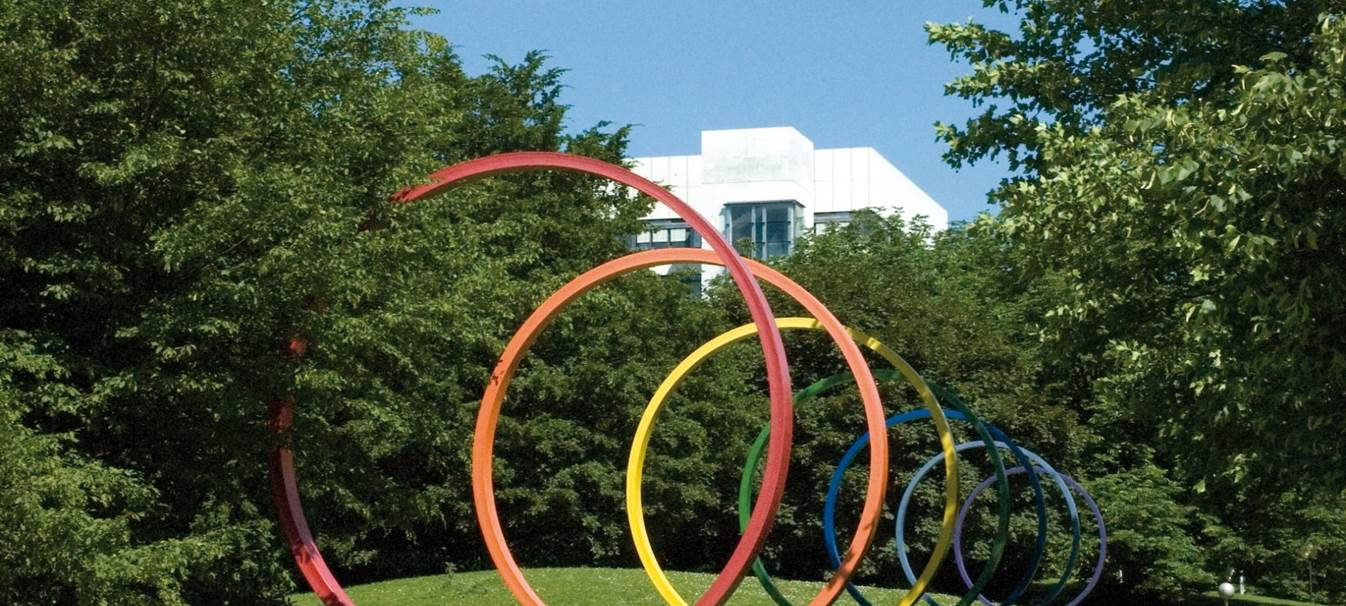
\includegraphics[width=0.7\textwidth]{images/tudo-title-2.jpg}}


\begin{document}

\maketitle

\section{The Cherenkov Telescope Array}


\begin{frame}{The Cherenkov Telescope Array}
    \begin{columns}[T] % align columns
        \begin{column}{.45\textwidth}
            \vspace{10pt}
            \begin{itemize}
                \item "Cherenkov Telescope Array"
                \item Proposed in 2005
                \item Currently in pre-production
                \item Two arrays of multiple telescopes
                \item Three types of telescopes: LST, MST, SST
                \item Goals: Extend observable energy range, higher sensitivity, huge field of view
                \item Status: First Crab Nebula observation with LST1
            \end{itemize}
        \end{column}%
        \hfill%
        \begin{column}{.53\textwidth}
            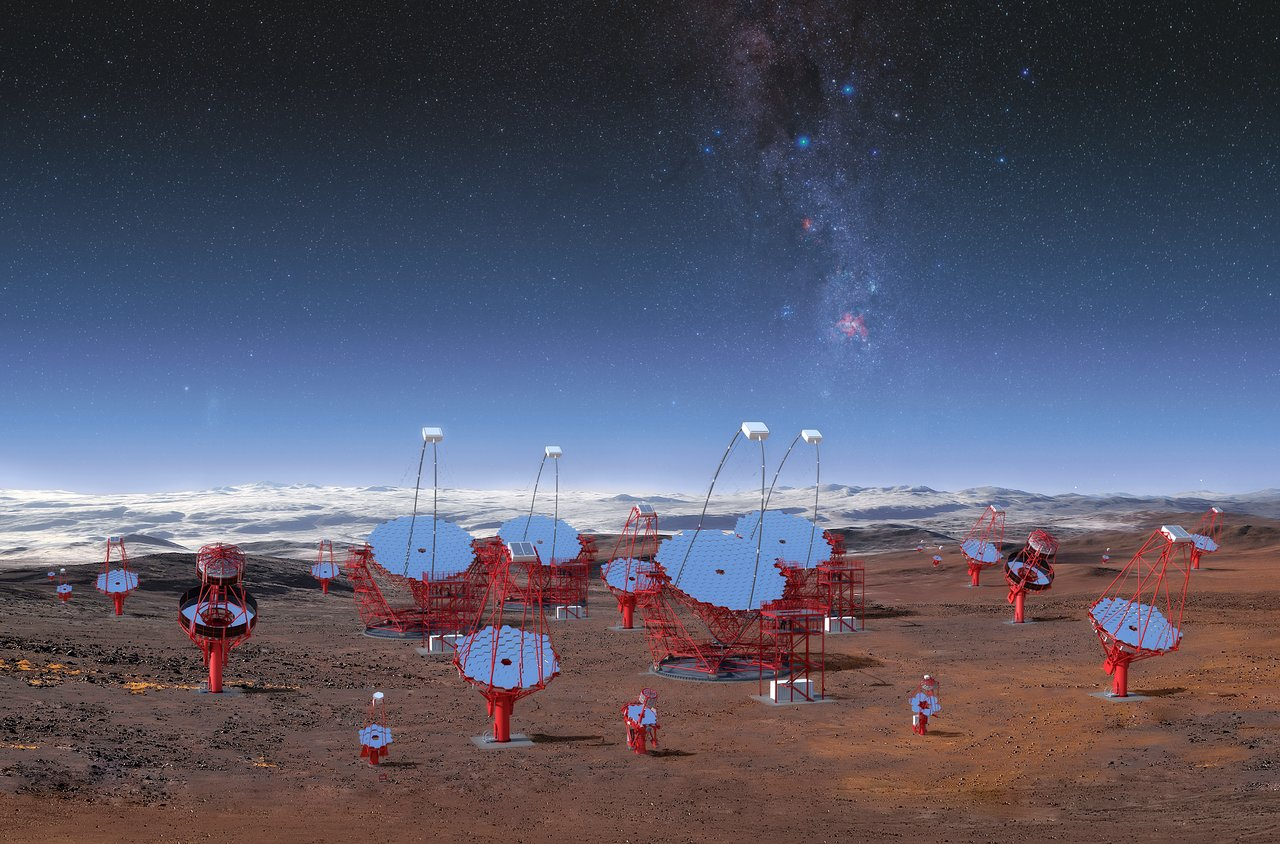
\includegraphics[width=\linewidth]{images/cta_telescopes.jpg}
            Visualization of the different telescope types.
            \cite{cta_telescopes}
        \end{column}%
    \end{columns}
    
\end{frame}



\begin{frame}{Layout}
      \begin{figure}
      \centering
       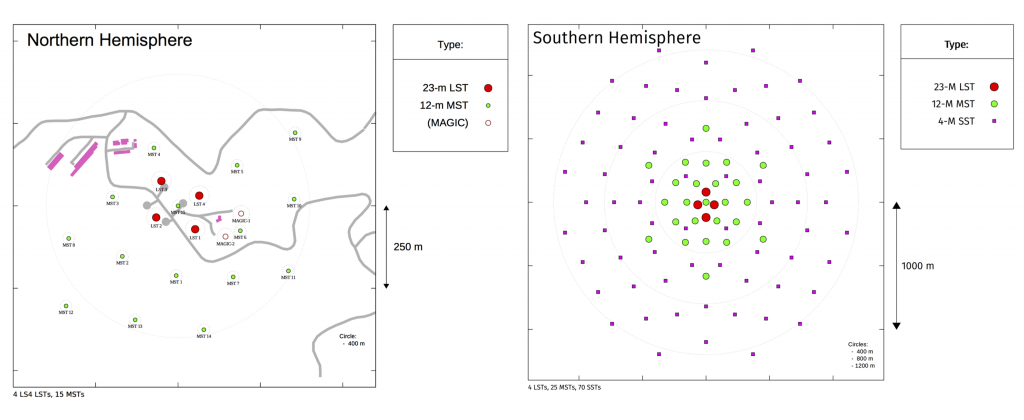
\includegraphics[width=\textwidth]{images/cta_layout.png}
      \end{figure}
\end{frame}

\begin{frame}{ctapipe}
    \begin{columns}[T] % align columns
        \begin{column}{.45\textwidth}
            \vspace{10pt}
            \begin{itemize}
                \item { Pipeline for low level cta data}
                \item { Coordinate transformation, calibration, cleaning, 
                        hillas-parameters, 3D-reconstruction, visualization}
                \item { Still in active development} 
                \item { Mainly \textbf{python} based}
                \item { https://github.com/cta-observatory/ctapipe}
            \end{itemize}
        \end{column}
        \begin{column}{.48\textwidth}
            
\includegraphics[width=\linewidth]{images/ctapipe_logo.png}
            
\includegraphics[width=\linewidth]{images/python_logo.png}
        \end{column}
    \end{columns}
\end{frame}




\section{Position Reconstruction}
\begin{frame}
  \centering
  {\Huge \textbf{Reconstruction of the source position}}
\end{frame}

\begin{frame}{Reconstruction}
  \begin{columns}[T]
    \begin{column}{.45\textwidth}
      HillasReconstructor:
      \begin{itemize}
        \item \geq 2 telescopes needed
        \item Geometric combination of "hillas planes"
        \item Scales very well with more telescopes
      \end{itemize}
      \begin{tikzpicture}[x  = {(0cm,-0.5cm)},
                          y  = {(1cm,0cm)},
                          z  = {(0cm,1cm)},
                          color = {lightgray},
                          scale = 0.6,
                          declare function = {
                            q(\x) = \x - 1;
                            Z(\x,\y) = 1;
                            w(\x,\y,\z) = \x^2 * (3 + 2*\x)*(1+\x*\y)*(1+\x*\z)/(1+\x^2);}
                            %exp(-( (x-\centerx)^2/\sigmax^2 + (y-\centery)^2/\sigmay^2 + (z-\centerz)^2/\sigmaz^2)/3);}
                        ]
        % style of faces
        \centering
        \begin{scope}
        %\tikzset{facestyle/.style={fill=lightgray,draw=red,very thin,line join=round}}

        \coordinate (A) at (4,0,0);
        \coordinate (B) at (2,2,0);
        \coordinate (C) at (1,3,4);
        \coordinate (A2) at (4,4,0);
        \coordinate (A3) at (0,0,0);
        \coordinate (A4) at (0,4,0);


        \def\tsize{0.23}
        \def\flength{0.28}

        \foreach \corner in {A,A2,A3,A4}{
          \coordinate (LST) at ($(\corner)!0.5!(B)$);
          
          \draw[draw=black, join=round, fill=lightgray]
            ($(LST)+(\tsize,-1*\tsize/2,0)$) --
            ($(LST)+(\tsize,\tsize/2,0)$) --
            ($(LST)+(\tsize/2,\tsize,0)$) --
            ($(LST)+(-1*\tsize/2,\tsize,0)$) --
            ($(LST)+(-1*\tsize,\tsize/2,0)$) --
            ($(LST)+(-1*\tsize,-1*\tsize/2,0)$) --
            ($(LST)+(-1*\tsize/2,-1*\tsize,0)$) --
            ($(LST)+(\tsize/2,-1*\tsize,0)$) --
            ($(LST)+(\tsize,-1*\tsize/2,0)$);

          \draw[draw=red, join=round, very thin]
            ($(LST)+(0,\tsize,0)$) --
            ($(LST)+(0,0,\flength)$)--
            ($(LST)+(0,-1*\tsize,0)$);

          \node[black] at 
            ($(LST)+(0,0,\flength)$)
            {\textbullet};

          \draw[fill=blue,draw=black,opacity=.1,very thin,line join=round]
            (\corner) -- 
            (B) --
            (C);
        }

        \draw[draw=black, ->]
        (B) --
        ($(B)!1.2!(C)$);

        \end{scope}


        % shower, this will need more work
        \begin{scope}
        \begin{axis}[
          axis line style={draw=none},
          tick style={draw=none},
          ticks=none]
        \def\centerx{1.5}
        \def\centery{2.5}
        \def\centerz{2}
        \def\sigmax{1}
        \def\sigmay{1}
        \def\sigmaz{1}
        \addplot3[
          surf,
          shader=faceted,
          samples=10,
          domain=0:4,y domain=0:4,
          z buffer=sort,
          opacity=0.15
        ]
        ({x*cos(deg(y))},{x*sin(deg(y))},{x});
        \end{axis}
        \end{scope}
        %\end{scope}
        % \begin{axis}
        % \addplot3[surf,domain=0:4,domain y=-5:3] 
        % {exp(-( (x-\centerx)^2 + (y-\centery)^2)/3 )};
        % \end{axis}
        % \node [red] at ($(A)!0.5!(B)$){\textbullet};
        % \node [red] at ($(A2)!0.5!(B)$){\textbullet};
        % \node [red] at ($(A3)!0.5!(B)!0.5!(B)$){\textbullet};
      \end{tikzpicture}

    \end{column}
    \begin{column}{.45\textwidth}
      disp:
      \begin{itemize}
        \item Mono at its core, different approaches for stereo mode
        \item Predicts a point on the main shower axis
      \end{itemize}
      \begin{figure}
        \centering
        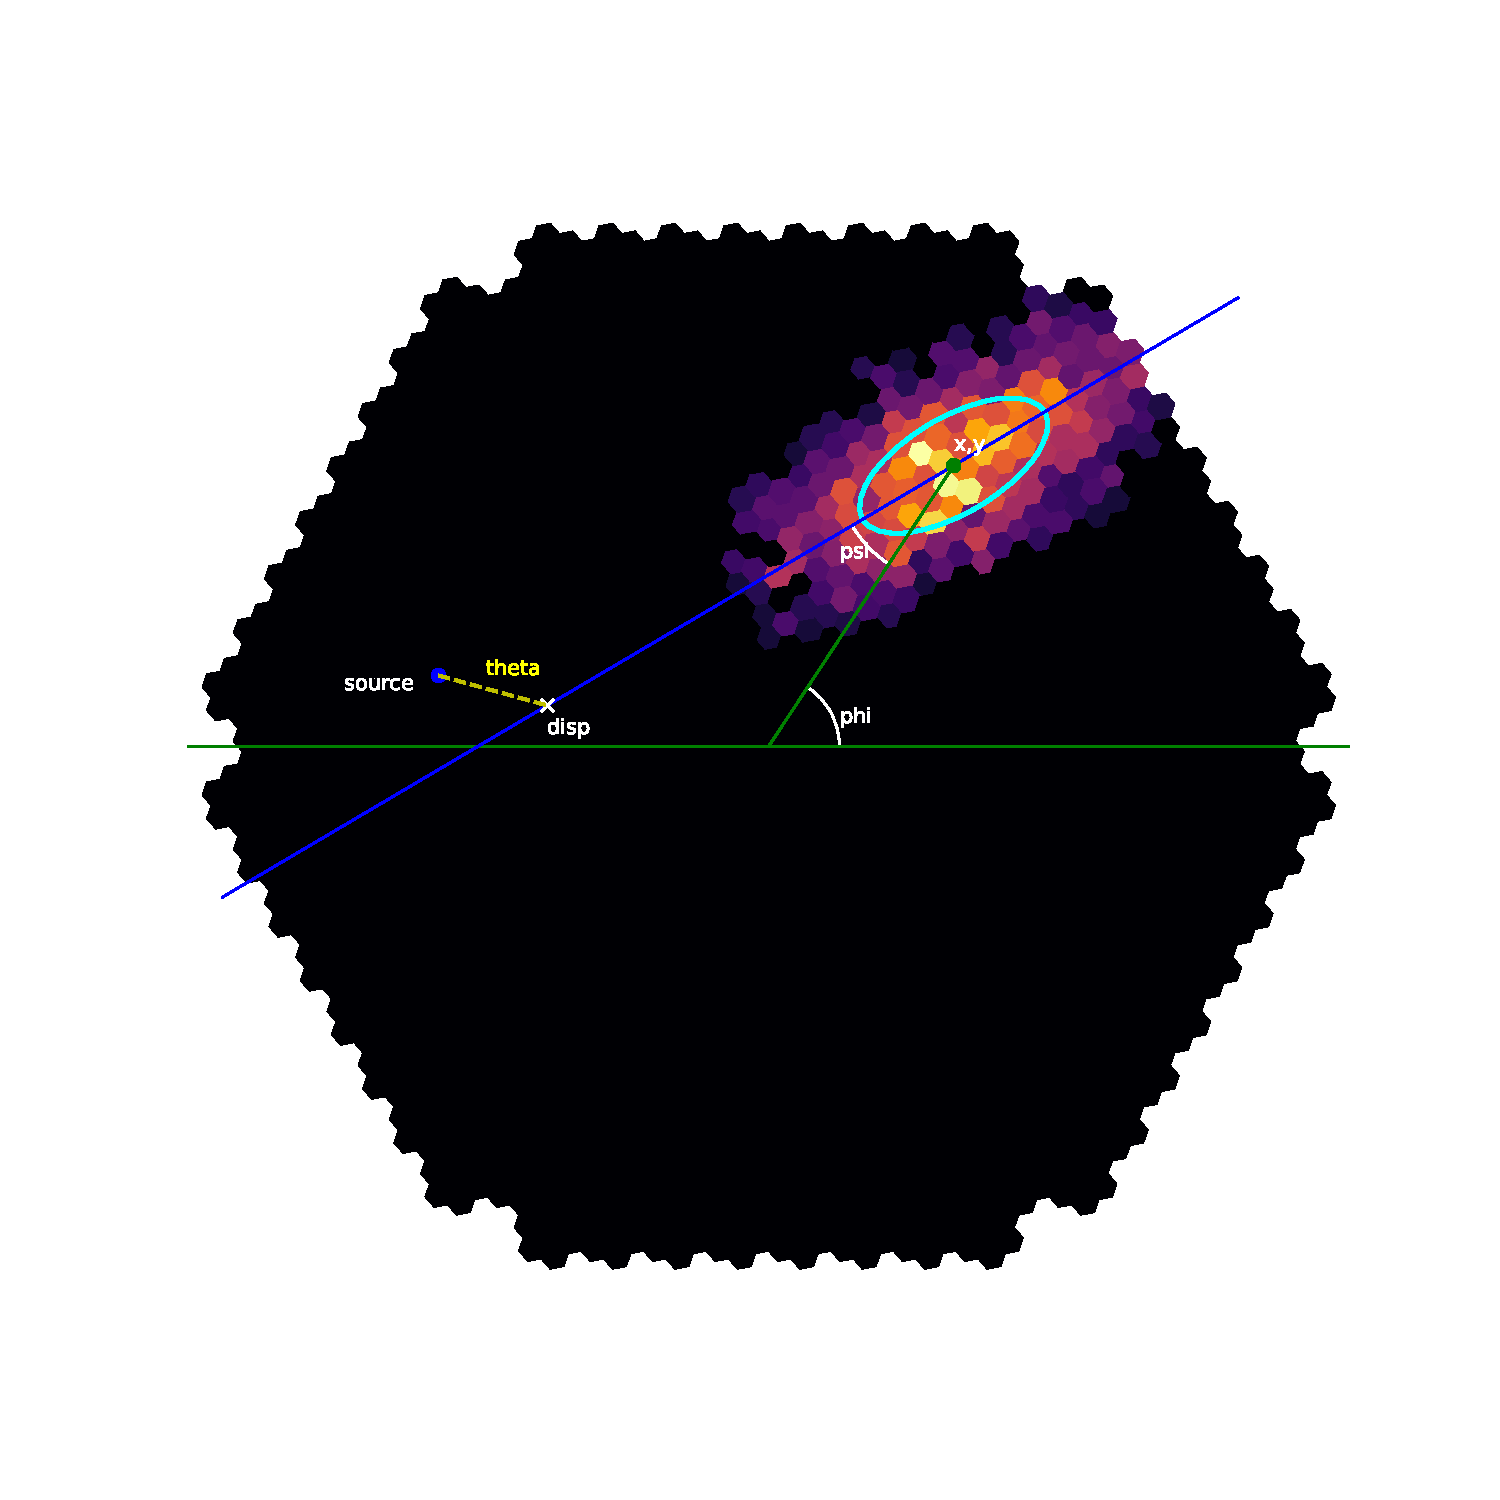
\includegraphics[width=0.8\textwidth]{../thesis/Plots/hillas_complete.pdf}
      \end{figure}
    \end{column} 
  \end{columns}
\end{frame}

%https://reader.elsevier.com/reader/sd/pii/S0927650515000316?token=BB3461639F455A5F5BC91247FB9D9BC210E98EF1CC4FF1A153145805FB7407B8E8E7488B12960C2F1307FF826190C6BF
\begin{frame}{magic disp}
  \begin{columns}[T]
    \begin{column}{.45\textwidth}
      \begin{itemize}
        \item 2 telescopes
        \item Stereo information to match the correct pair
        \item Uses either the intersection of the main shower axis or closest pair of points. -> paper 
      \end{itemize}
    \end{column}
    \begin{column}{.45\textwidth}
      Magic DISP-Abbildung! -> Paper!
    \end{column} 
  \end{columns}
\end{frame}


\section{Application to CTA MC-data}
\begin{frame}
  \centering
  {\Huge \textbf{Application to CTA MC-data}}
\end{frame}

\begin{frame}{Scaling of the MAGIC-DISP approach} % naming
  \begin{columns}[T]
    \begin{column}{.45\textwidth}
      \begin{itemize}
        \item identify all pairs of telescopes
        \item for each pair: find the closest two predictions and append them to our list
        \item average over that list, median here, weighted mean would be possible, but mean seems to be worse than median
      \end{itemize}
    \end{column}
    \begin{column}{.45\textwidth}
      \animategraphics[loop,controls,width=\linewidth]{10}{../thesis/Plots/stereo_magic_}{1}{6} %%% save as png
    \end{column} 
  \end{columns}
\end{frame}

\begin{frame}{Analysis}
  \begin{itemize}
    \item tons of prod3 data, south array
    \item ctapipe 63fe206b1d603b0fff61486b6d0c18f73ef4e321, basically 0.6.1
    \item some standard preprocessing, explain that stuff, cite kai
    \item high level analysis with aict tools, cite that, did some cta compatibility stuff, no standard cta format is problematic for support
  \end{itemize}
\end{frame}

\begin{frame}{Results}
  \begin{itemize}
    \item mono out of competition, weird amount of sign mismatch, maybe do mono on lst only?
    \item n=2 is superior and is equal to magic analysis
    \item n>3 gets worse quickly, not much to do
  \end{itemize}
%  mehrere Folien mit Plots: Disp results: acc/R2, vs Energy, vs. Multiplicity, vs. Energy bei Multiplicity 2 und/oder 3 
\end{frame}

\begin{frame}
  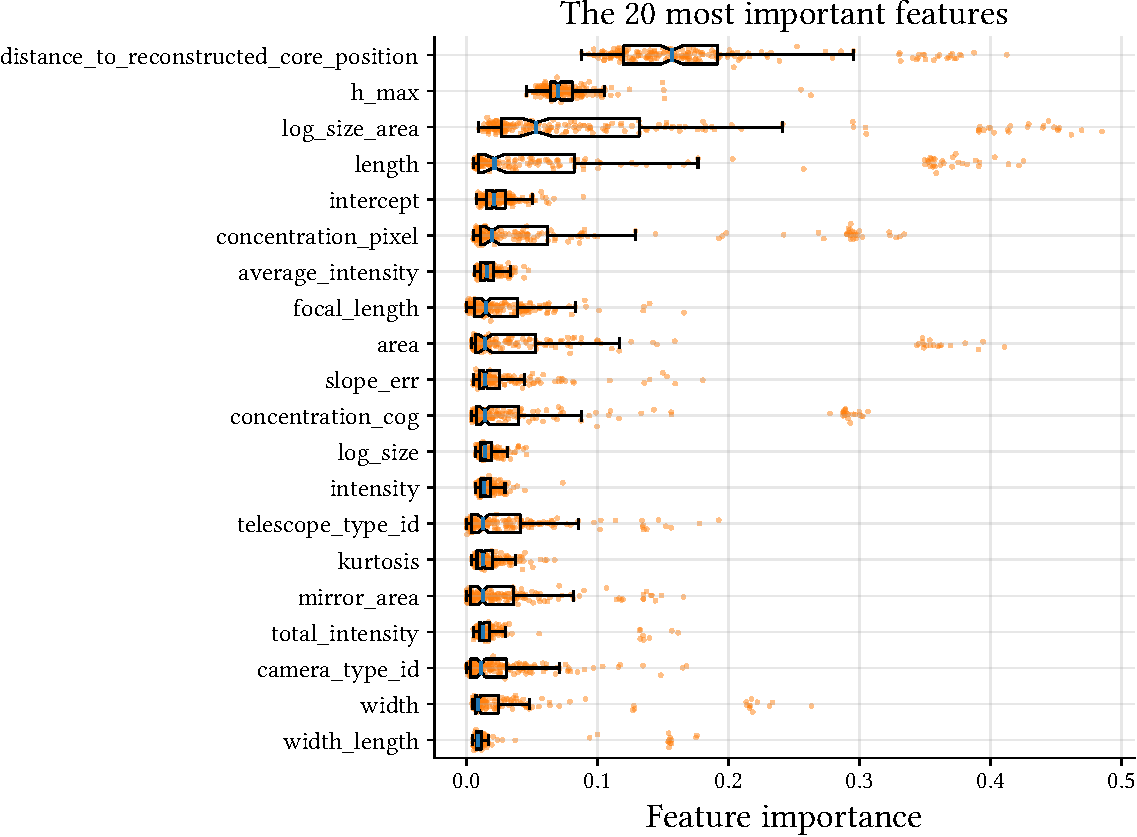
\includegraphics[width=0.7\textwidth]{../analysis/plots/disp_features.pdf}
\end{frame}

\begin{frame}{disp features}
  \begin{columns}[T]
    \begin{column}{.45\textwidth}
      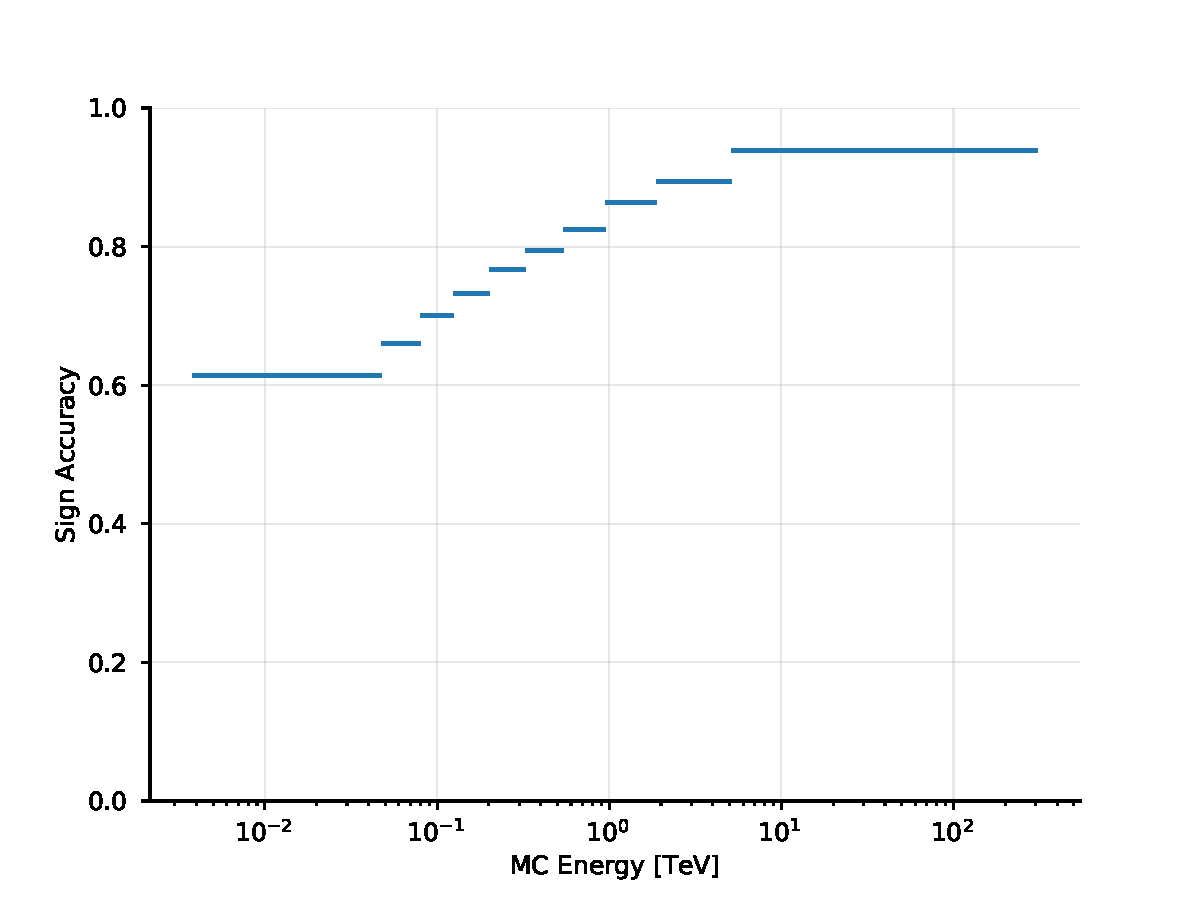
\includegraphics[width=\textwidth]{../analysis/plots/disp_accuracy_gamma.pdf}
    \end{column}
    \begin{column}{.45\textwidth}
      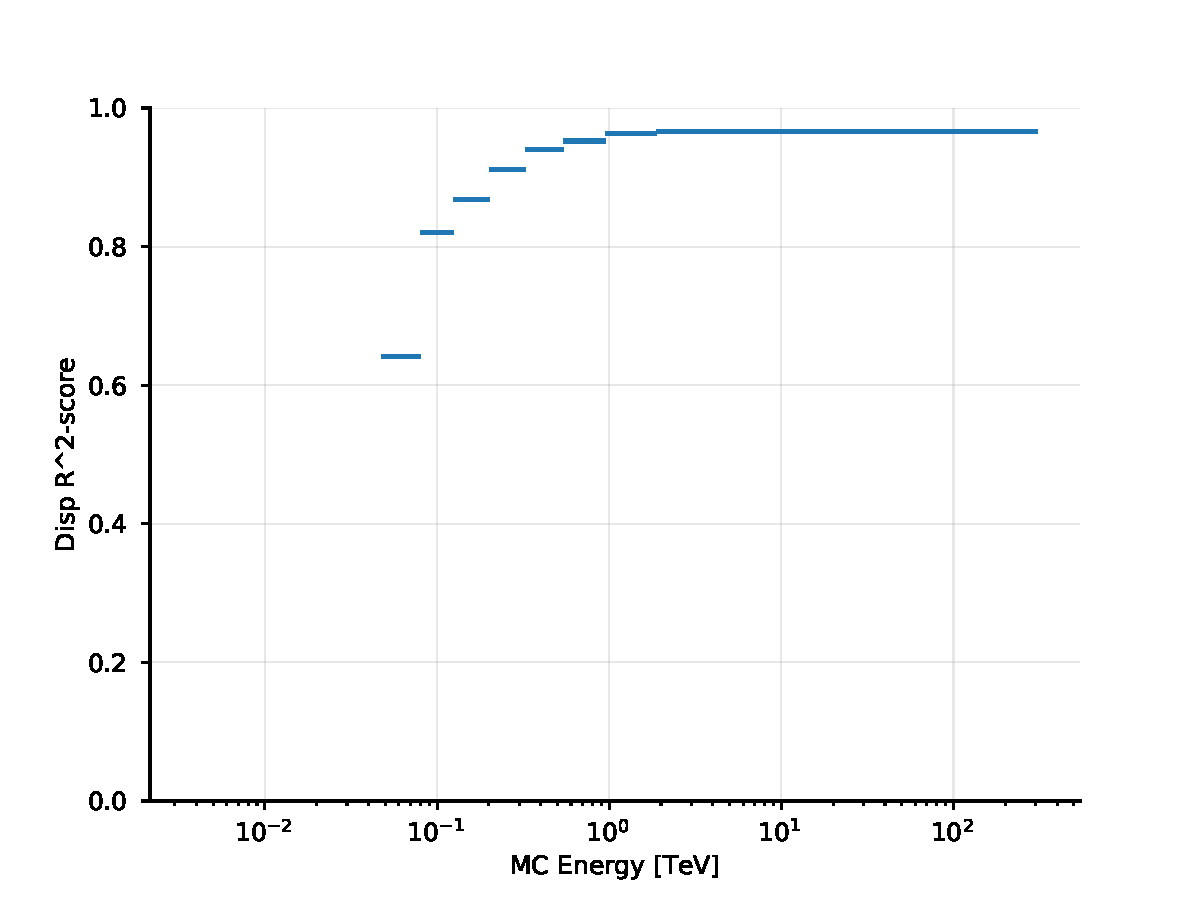
\includegraphics[width=\textwidth]{../analysis/plots/disp_r2_gamma.pdf}
    \end{column} 
  \end{columns}
\end{frame}

\begin{frame}
  \begin{figure}
    \centering
    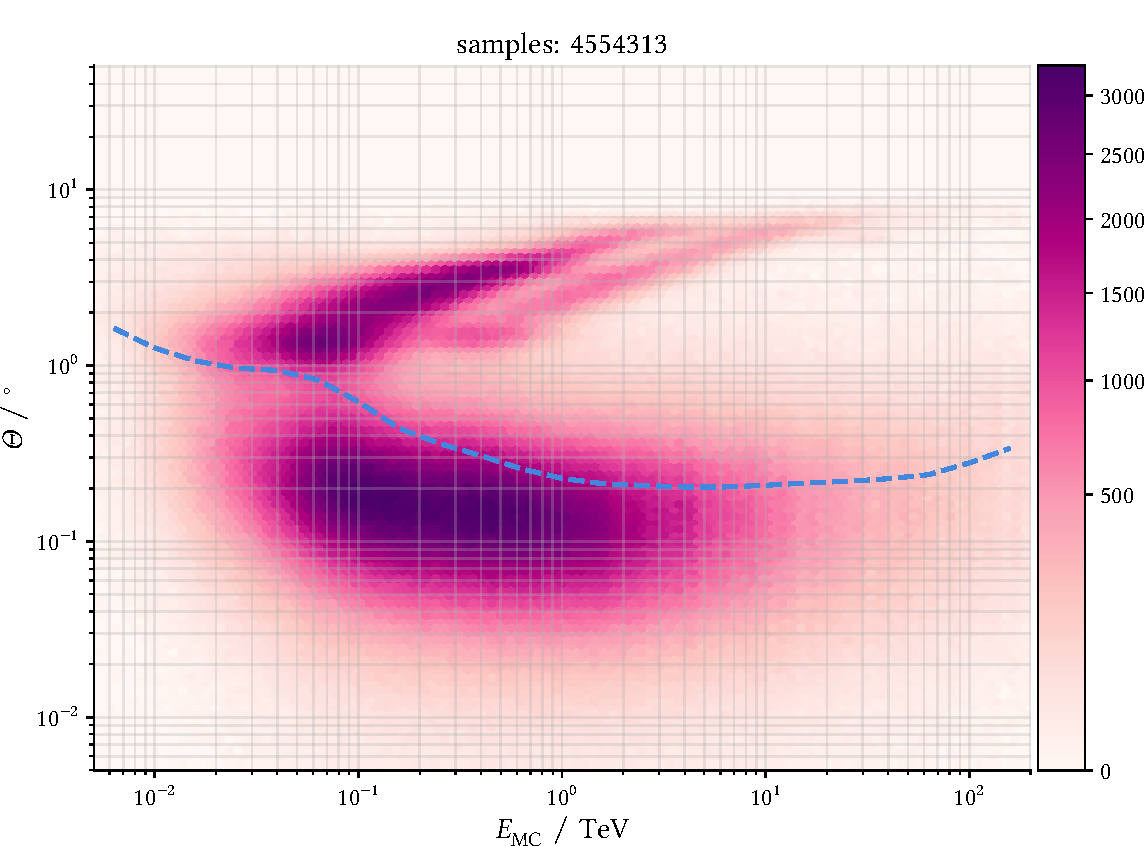
\includegraphics[width=0.6\textwidth]{../analysis/plots/gamma/tel_vs_energy.pdf}
  \end{figure}
\end{frame}

\begin{frame}
  \begin{columns}[T]
    \begin{column}{.45\textwidth}
    % bins are from disp!
      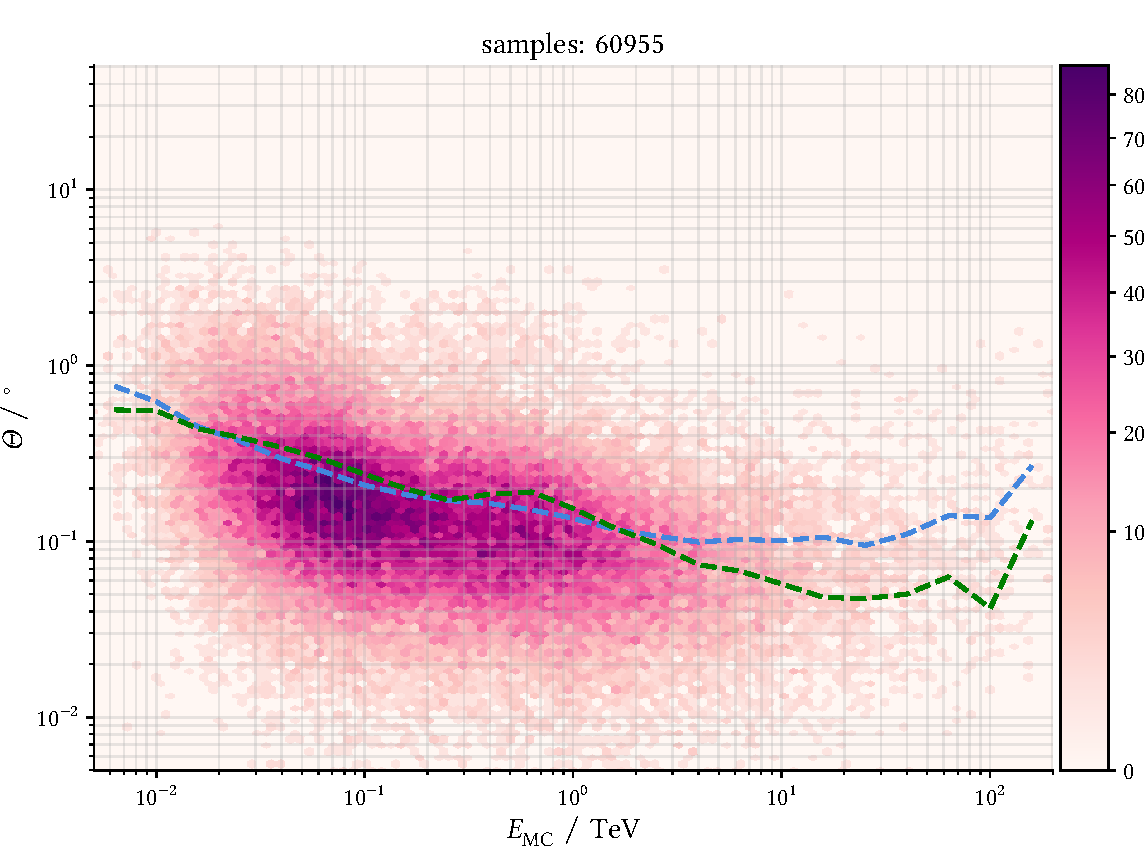
\includegraphics[width=\textwidth]{../analysis/plots/gamma/pairwise_median_100_vs_energy.pdf}
    \end{column}
    \begin{column}{.45\textwidth}
      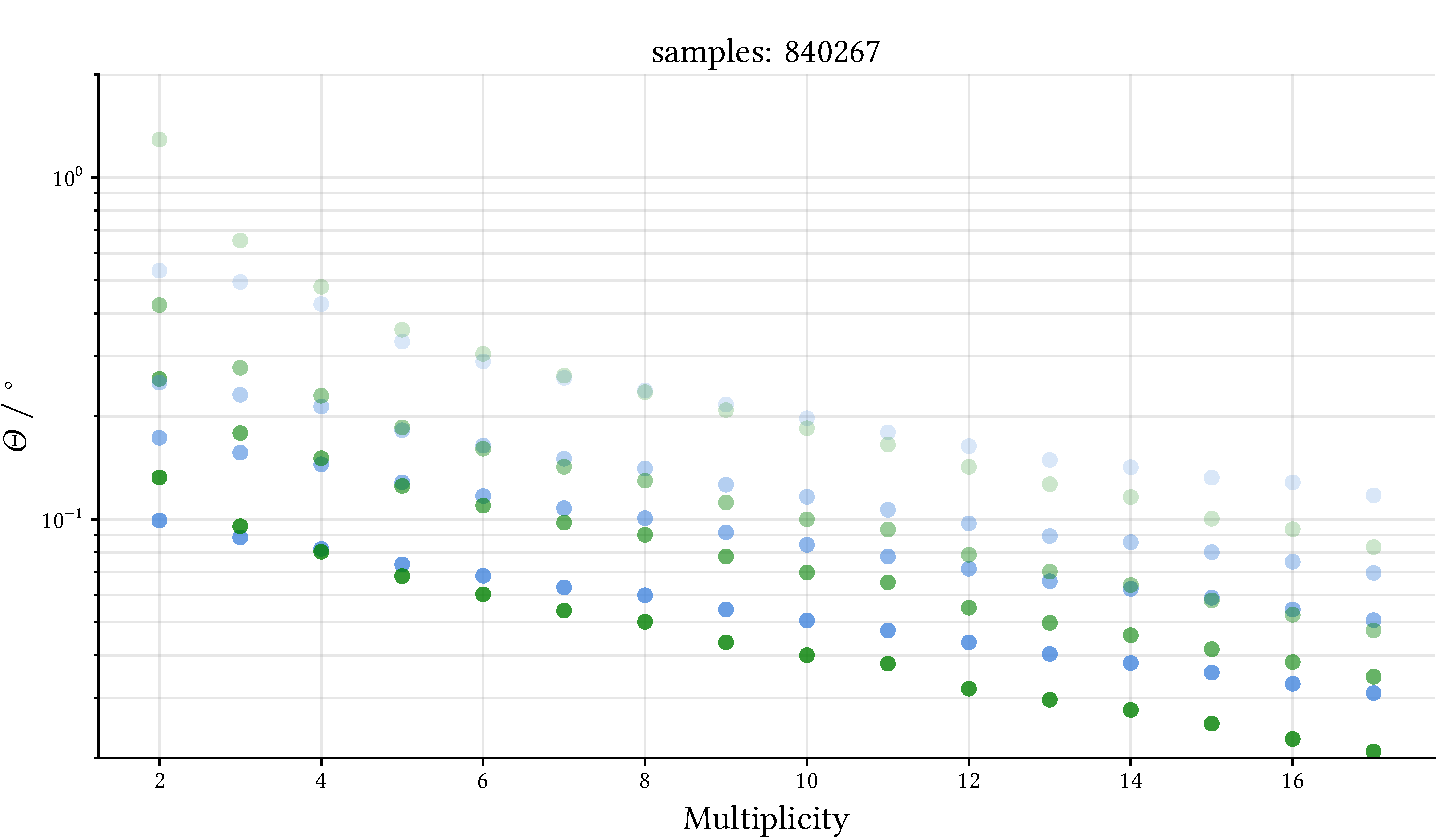
\includegraphics[width=\textwidth]{../analysis/plots/gamma/pairwise_median_100_vs_multi_comp.pdf}
    \end{column} 
  \end{columns}
\end{frame}

\begin{frame}{summary}
  \begin{itemize}
    \item somewhat useful, but not that much
  \end{itemize}
\end{frame}

\begin{frame}
    \centering
    {\Huge \textbf{Thank you for your attention!}}
\end{frame}

\begin{frame}{bib}
  bib stuff, use refernce from thesis 
\end{frame}

\end{document}